\documentclass[oneside]{ausarbeitung}
\bibliography{latexlit}


% ----------------------------------------------------------------------

\begin{document}

%--- Sprachauswahl
% Erlaubte Werte:
%   \selectlanguage{english}
%   \selectlanguage{ngerman}
\selectlanguage{ngerman}

%--- Art der Arbeit
% Erlaubte Werte:
%   \Praxissemesterbericht
%   \Projektbericht
%   \Bachelorarbeit
%   \Seminararbeit
%   \Masterarbeit

\Projektbericht

%--- Studiengang:
% Erlaubte Werte:
%   \Informatik
%   \Elektronik
%   \DataScience
\Informatik

\title{Algorithmisches Handeln von Kryptowährungen}

\author{Sebastian Flum}
\matrikelnr{76855}

%--- Ist der Erstbetreuer (\examinerA) an der Hochschule ein Professor?
% Erlaubte Werte:
%   \examinerIsAProfessortrue   % Ja
%   \examinerIsAProfessorfalse  % Nein
\examinerIsAProfessorfalse

%--- Betreuer
\examinerA{Sebastian Stigler}
%\examinerB{Prof.~Dr.~Ulrich~Klauck}

%--- Einreichungsdatum
\date{28. Februar 2021}

%--- Titelseite Anzeigen
\maketitle
\cleardoublepage

%---
\pagenumbering{roman}
\setcounter{page}{1}

%--- Eidesstattliche Erklärung anzeigen
\makeaffirmation
\cleardoublepage

%---
\begin{abstract}

Beim algorithmischen Handeln werden Handelsentscheidungen auf der Grundlage zuvor definierter Anweisungen und Regeln getroffen, die in Form eines Computerprogramms umgesetzt wurden. Dabei wird Code geschrieben, der die Trades im Namen des Händlers oder Investors ausführt, wenn bestimmte Bedingungen erfüllt sind. 

Im Rahmen dieser Arbeit wurde versucht, jenes Verfahren auf den Handel von kryptographischen Währungen wie Bitcoin oder Ethereum anzuwenden und ein algorithmisches Handelssystem für diese zu entwerfen. So soll herausgefunden werden, ob der automatisierte Handel von Kryptowährungen, durch ein selbst entwickeltes System, erfolgreich sein kann.

Dabei beschäftigt sich diese Arbeit im grundlegenden mit folgenden Konzepten:

\begin{enumerate}
	\item Algorithmische Handelsstrategien und technische Indikatoren
	\item Implementierung einer Schnittstelle für Handelsplattformen
	\item Backtesting von Handelsstrategien
	\item Erstellung einer Konsolenanwendung
	\item Verknüpfung dieser Elemente innerhalb eines modularen Systems
\end{enumerate}

Umgesetzt wurde dieses Projekt fast ausschließlich unter der objektorientierten Verwendung der Programmiersprache Python, in Verbindung mit einigen wenigen HTML Elementen.

\end{abstract}
%-----------------------------------------------------------------------
\cleardoublepage
\tableofcontents

%---
\listoffigures

%---
\listoftables

%---
\listoflistings

%---
\listofabbreviations
\begin{acronym}[Bsp.]  % Längstes Kürzel in der nachfolgenden
                       % Liste um die Breite der Spalte für die
                       % Abkürzungen zu bestimmen.

%% Eintrag: \acro{Referenzname}[Kürzel]{Langform}
%% Im Text wird die Abkürzung dann mit \ac{Referenzname} benutzt.
\acro{rup}[RUP]{Rational Unified Process}
\acro{bsp}[Bsp.]{Beispiel}
\end{acronym}
%---


\cleardoublepage
\pagenumbering{arabic}
\setcounter{page}{1}

% ----------------------------------------------------------------------
\chapter{Einleitung}
\label{cha:einleitung}

"Neues Allzeithoch: Bitcoin-Rekordjagd geht ungebremst weiter".\cite{bitcoin_artikel_1} "Kryptowährung: Bitcoin knackt Marke von 50.000 Dollar".\cite{bitcoin_artikel_2} Artikel wie diese sind schon lange keine Seltenheit mehr. Kryptowährungen, allen voran der Bitcoin, entwickelten sich in den letzten Jahren zum Sinnbild schnellen Reichtums. Doch das war nicht immer so. Im Jahre 2011, als sich der Bitcoin noch in seinen Kinderschuhen befand, kostete ein Coin gerade einmal 1 Dollar.\cite{bitcoin_kurs_2011} Vielleicht erwischt man sich nun selbst bei dem Gedanken daran, was wohl wäre, wenn man zu dieser Zeit schon das Potential dieser, damals unscheinbaren, Internetwährung erkannt hätte. Einige vorausdenkende Köpfe erkannten dies frühzeitig und wurden dadurch reich. Andere wiederum nutzten die neu entdeckte Kryptowährung dazu, online für ihre Pizza zu bezahlen. Verrückt, wenn man sich vor Augen führt, dass man mit der selben Menge Bitcoins heute zehntausende Pizzen bezahlen könnte. Vielleicht lässt dieser Gedanke die Herzen einiger Pizzaliebhaber höher schlagen, vorrangig stellt sich jedoch die Frage, ob man mit dem Besitz und Handel von Kryptowährungen heutzutage noch Erfolg haben kann. Und wenn ja - kann das auch ein Computerprogramm?

\section{Motivation}
\label{sec:motivation}



In der Motivation wird dargestellt, welche Bedeutung die im 
Praxissemester zu entwickelnden Lösungen für das betreuende Unternehmen 
haben. Es wird beispielsweise aufzeigt, in welches Produkt sie eingehen, 
welcher Ablauf verbessert werden soll etc.

\section{Problemstellung und -abgrenzung}
\label{sec:problemstellung}

Die Problemstellung dient dazu, das zu lösende Problem klar zu 
definieren und abzugrenzen. Der Praktikant soll ein klares Verständnis 
des zu lösenden Problems haben. Insbesondere soll auch verhindert 
werden, dass zu viele Probleme gleichzeitig angegangen werden. Eine 
Negativabgrenzung verhindert, dass beim Leser später nicht erfüllte 
Erwartungen geweckt werden.

\section{Ziel der Arbeit}
\label{sec:ziel}

Mit dem Ziel der Arbeit wird der angestrebte Lösungsumfang festgelegt. An diesem Ziel wird entschieden, ob das Praktikum erfolgreich absolviert wurde oder nicht.

\section{Vorgehen}
\label{sec:vorgehen}

Nachdem mit Problemstellung und Ziel gewissermaßen Anfangs- und Endpunkt 
des Praktikums beschrieben sind, wird hier der zur Erreichung des Ziels 
eingeschlagene Weg vorgestellt. Dazu werden typischerweise die folgenden 
Kapitel und ihr Beitrag zur Erreichung des Ziels der Arbeit kurz 
beschrieben. Die folgenden Kapitel sind ein – möglicher – Aufbau, 
Abweichungen können durchaus notwendig sein. Zur Darstellung des 
Vorgehens ist eine grafische Darstellung sinnvoll, bei der die einzelnen 
Lösungsschritte und ihr Zusammenhang dargestellt werden. Ein Beispiel 
hierfür findet sich in Abbildung \ref{fig:1}.

\begin{figure}[htbp]
  \centering
  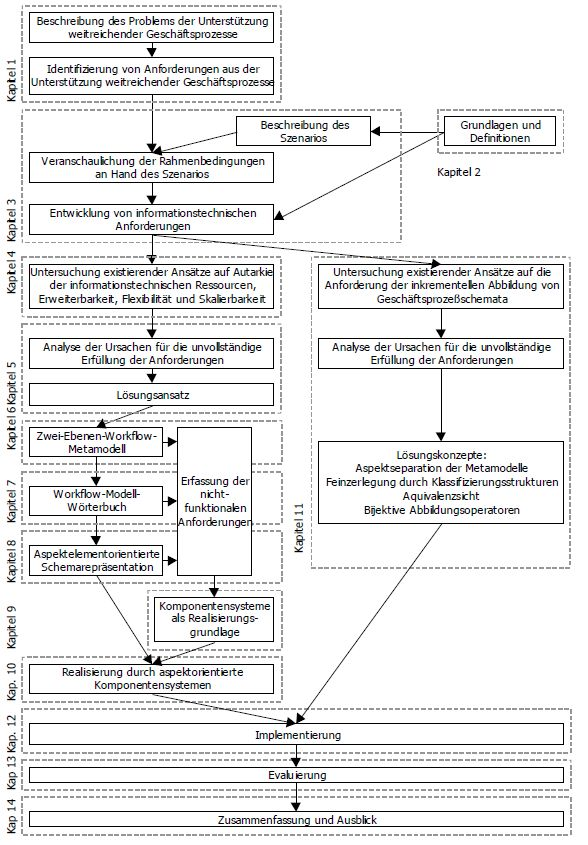
\includegraphics[height=0.9\textheight]{img/ausarbeitung.jpg}
  \caption{vorgehen nach \autocite{Schmidt:Geschaeftsprozesse}}
  \label{fig:1}
\end{figure}


% ---
\chapter{Grundlagen}
\label{cha:grundlagen}

In diesem Kapitel das für das Praktikum relevante Grundlagenwissen 
dargestellt. Der Praktikant soll hierzu das ihm durch Vorlesungen 
bekannte, bzw. durch Recherchen vertiefte theoretische Wissen 
darstellen, das für die Lösung der im Praktikum gestellten Probleme 
notwendig ist.

Dabei ist darauf zu achten, nur solche Inhalte in das Grundlagenkapitel 
aufzunehmen, die später auch verwendet werden (Problembezogenheit). 
Ebenso ist auf eine ausreichend tiefe und vollständige Darstellung der 
Grundlagen zu achten.

Für die Erstellung des Literaturverzeichnisses 
wird das Werkzeug JabRef\autocite{JabRef:JabRef} verwendet. 

Sie können aber auch das Werkzeug Citavi\autocite{SAS:Citavi} benutzen
und dort nach \textsc{Bib}\TeX{} exportieren.

\section{Grundlagengebiet A}
\label{sec:grundlagengebieta}

\subsection{Definition AA}
\label{sub:definitionaa}

\subsection{Definition AB}
\label{sub:definitionab}

\section{Grundlagengebiet B}
\label{sec:grundlagengebietb}

\subsection{Definition BA}
\label{sub:definitionBa}

\subsection{Definition BB}
\label{sub:definitionbb}

%---
\chapter{Problemanalyse}
\label{cha:problemanalyse}

Die Analyse des zu lösenden Problems ist Grundlage für jedes 
ingenieurmäßige Vorgehen. Daher soll in diesem Kapitel das zu lösenden 
Problem auf Basis des im Grundlagenkapitel aufbereiteten Wissens 
analysiert werden. Hierzu ist insbesondere notwendig zu klären, wie sich 
das Gesamtproblem in Teilprobleme zerlegen lässt und welche 
Abhängigkeiten zwischen diesen bestehen.

Bei Software-Projekten befindet sich an dieser Stelle typischerweise die 
Anforderungsanalyse des \ac{rup}.

%---
\chapter{Lösungskonzept}
\label{cha:loesungskonzept}

Auf der Basis der im vorangegangenen Kapitel erstellten Problemanalyse 
und der im Grundlagenkapitel aufgearbeiteten theoretischen Kenntnisse 
wird ein Lösungskonzept erarbeitet.

Bei Software-Projekten entspricht dieses Kapitel typischerweise der 
Analyse \& Design-Phase des \ac{rup}. Typische Ergebnisse dieser Phase sind 
Klassendiagramme etc.

%---
\chapter{Implementierung}
\label{cha:implementierung}

In diesem Kapitel wird die konkrete Implementierung des im Kapitel
\ref{cha:loesungskonzept} entwickelten Lösungskonzepts beschrieben.
Hierbei wird auf die konkret verwendeten Entwicklungswerkzeuge etc. 
Bezug genommen.

Bei Software-Projekten besteht dieses Kapitel typischerweise aus den 
Phasen Implementierung \& Test im \ac{rup}.

Zum Beispiel kann man hier auch ein kleines Listing einfügen.

\begin{lstlisting}[language=c,%
                   caption={Überschrift des Quelltexts}]
#include<stdio.h>

int main() {
    // Kommentar
    int answer = 20 << 1;
    answer += 2;
    printf("Hallöchen Welt!\n");
    printf("Die Antwort ist: %d\n", answer);
    return 0;
}
\end{lstlisting}

Manchmal hilft auch eine kleine Tabelle:

\begin{table}[htbp]
\centering
\begin{tabular}{|l|r|}
\hline
\textbf{Messwert a} & \textbf{Messwert b} \\ \hline
9 & 5 \\ \hline
1 & 4 \\ \hline
1 & 3 \\ \hline
\end{tabular}
\caption{Überschrift der Tabelle}
\label{tab:my-table}
\end{table}

Details siehe Tabelle~\ref{tab:my-table}.
%---
\chapter{Inbetriebnahme}
\label{cha:inbetriebnahme}

Aufgabe des Kapitels Inbetriebnahme ist es, die Überführung der in 
Kapitel \ref{cha:implementierung} entwickelte Lösung in das betriebliche 
Umfeld aufzuzeigen. Dabei wird beispielsweise die Inbetriebnahme eines 
Programms beschrieben oder die Integration eines erstellten 
Programmodules dargestellt.

Bei der Software-Erstellung entspricht dieses Kapitel der 
Auslieferungsphase (Deployment) im \ac{rup}.

%---
\chapter{Evaluierung}

Aufgabe des Kapitels Evaluierung ist es, in wie weit die Ziele der 
Arbeit erreicht wurden. Es sollen also die erreichten Arbeitsergebnisse 
mit den Zielen verglichen werden. Ergebnis der Evaluierung kann auch 
sein, das bestimmte Ziele nicht erreicht werden konnten, wobei die 
Ursachen hierfür auch außerhalb des Verantwortungsbereichs des 
Praktikanten liegen können.

%---
\chapter{Zusammenfassung und Ausblick}
\label{cha:zusammenfassung}

\section{Erreichte Ergebnisse}
\label{sec:ergebnisse}

Die Zusammenfassung dient dazu, die wesentlichen Ergebnisse des 
Praktikums und vor allem die entwickelte Problemlösung und den 
erreichten Fortschritt darzustellen. (Sie haben Ihr Ziel erreicht und 
dies nachgewiesen).

\section{Ausblick}
\label{sec:ausblick}

Im Ausblick werden Ideen für die Weiterentwicklung der erstellten Lösung 
aufgezeigt. Der Ausblick sollte daher zeigen, dass die Ergebnisse der 
Arbeit nicht nur für die in der Arbeit identifizierten Problemstellungen 
verwendbar sind, sondern darüber hinaus erweitert sowie auf andere 
Probleme übertragen werden können.

\subsection{Erweiterbarkeit der Ergebnisse}
\label{sub:erweiterbarkeit}

Hier kann man was über die Erweiterbarkeit der Ergebnisse sagen.

\subsection{Übertragbarkeit der Ergebnisse}
\label{sub:uebertragbarkeit}

Und hier etwas über deren Übertragbarkeit.

%-----------------------------------------------------------------------
\appendix

%---
\printbibliography[heading=bibintoc]

%---
\chapter{Anhang A}

%---
\chapter{Anhang B}


\end{document}